\section{Feedback}
\subsection{Risks}
 A part of project management and a the project manager's responsability of is to be able to anticipate the risks of the project. A major issue would be to let the daily events and issues drive the project lifetime. The project manager must be pro-active and produce a risk chart.

As we knew nothing about the topic we were going to work on and we were not really experienced in Fortran and MPI, we originaly anticipate onthe following riks.

\begin{tabular}{ | p{0.09\textwidth} |  p{0.91\textwidth} |}
\hline
\textbf{Definition} & \textbf{Probability} & \textbf{Impact} & \textbf{Action}
\\

\hline
The product do not fit the client expectation. &
\textcolor{green}{Light} &
\textcolor{red}{Heavy} &
Specification with the client \\

\hline
Ressources inadequate &
\textcolor{orange}{Medium} &
\textcolor{red}{Heavy} &
Lighter test creation, request access on computers \\

\hline
Insufficiente knowledge &
\textcolor{red}{Heavy} &
\textcolor{red}{Heavy} &
Increase the time dedicated to each risky task \\
\hline
\end{tabular}


\subsection{Final Schedule}

Giving the risks anticipated we succesfully avoid some issues. However, we did'nt anticipated enough on the time spend to debug and to handle MPI library for one part and to refactore the code for a second part. Consequently the initial schhedule haven't been precisely observed and we get the following schedule. \\

\begin{figure}[h!]
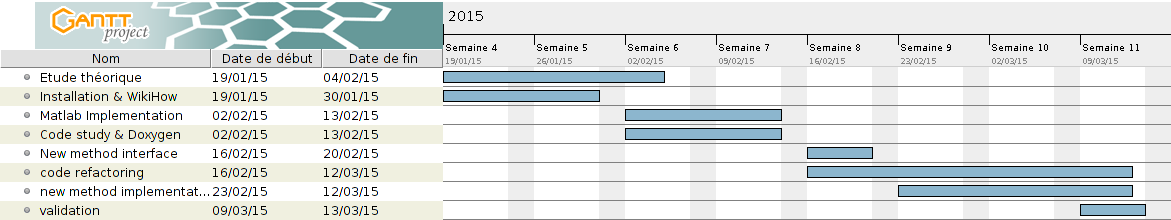
\includegraphics[width=1\textwidth]{Image/gantt2.png}\centering
\caption{\textit{Final gantt}}
\end{figure}

